\documentclass[oneside,a4paper,links]{cilamce2011}
%\documentclass[oneside,a4paper,writinenglish,links]{cilamce2011}
%
\usepackage{graphicx}
\usepackage{amsmath,amsfonts}
\usepackage{subfigure}

% Bruno: Command added to present problem in 'theorem form'
\newtheorem{problem}{Problem}

\title{Automated Finite Element Computation of the Pressure Equation for Porous Media Flow Using Convergence Acceleration via Multigrid}

\author[\voidaffil]{Bruno G. B. Luna}
\author[\voidaffil]{Paulo R. M. Lyra}
\author[\voidaffil]{Ramiro B. Willmersdorf}
%
\affil[\voidaffil]{Department of Mechanical Engineering, Federal University of Pernambuco, Cidade Universit\'aria s/n, Recife, PE, Brazil, \url{http://www.ufpe.br}}
%
%% NOTE: IF ALL AUTHORS BELONG TO THE SAME AFFILIATION
%% USE THE `\voidaffil' MACRO FOR THE AFFILIATION CODE.
%% Example:
%% \author[\voidaffil]{First A. Author}
%% \author[\voidaffil]{Second B. Author}
%% \author[\voidaffil]{Third C. Author}
%% \author[\voidaffil]{Fourth D. Author}
%% %
%% \affil[\voidaffil]{PROPEC, Department of Civil Engineering, School of Mines, 
%% Federal University of Ouro Preto, Campus Universit\'ario s/n,
%% Morro do Cruzeiro, 35400-000, Ouro Preto, MG, Brazil, http://www.propec.ufop.br}

\begin{document}
\vspace{3cm}

\maketitle

\begin{keywords}
Porous Media, Automatic Modeling, FEM.
\end{keywords}

\begin{abstract}
The simulation of multiphase flows in porous media imposes many numerical challenges
due to a number of factors such as the high anisotropic and heterogeneous media handled in this
type of analysis, the coupled elliptic-hyperbolic (or parabolic-quasi-hyperbolic) mathematical nature of the associated
Partial Differential Equations (PDEs), among others. One of the main difficulties faced
by numerical simulations of PDEs is the CPU time required for the solution of large systems of linear equations.
Multigrid methods allow a faster convergence of linear and non-linear equations systems
solvers. However, they normally require a sequence of progressive coarser meshes whose
generation can become an issue if not adequately addressed. Originally this sequence has
been made by setting different levels of refinement, manually or automatically, starting with
the coarsest mesh. Nevertheless this approach often leads to difficulties in representing
the geometrical details in the first mesh. It can also demand successive searches in
order to perform interpolations between different mesh levels, introducing extra errors. An alternative
to overcome these problems is to generate all the mesh hierarchy in a full algebric
manner using the so-called Algebraic Multigrid (AMG) approach. This work presents
the implementation of a software created using the \emph{FEniCS} tool for automated low-level
code generation and \emph{PyAMG} for the fully automatic creation of consistent multilevel
matrix structures to be applied to the numerical solution of the pressure equation that describes single phase porous media flows using the
Finite Element Method (FEM). The methods described here are general enough to handle
with three-dimensional, heterogeneous and anisotropic problems. Examples are shown
and results discussed for a two-dimensional problem in a heterogeneous domain with anisotropic permeability tensors.
\end{abstract}

\section{INTRODUCTION}
Nowadays, the numerical simulation of fluid flow in porous media is fundamental in many engineering fields, such as in the analysis of groundwater flow and contaminant transport \citep{Bear1992}, management of water and heat in polymer membranes for fuel cells \citep{Matamoros2006} or for the simulation of multiphase flows in petroleum reservoirs \citep{Peaceman1977, Aziz1979,Ewing1983,Carvalho2005,Silva2008}.

The scientific modeling of fluid flow in porous media for the petroleum industry has been done since the 1930's, initially using sand-packed models to understand the production of water in oil reservoirs and the reason why the water-oil rate increases with time. In the late 1930's and 1940's some experiments with electrolytic models were used to model the flow in porous media, as it was already recognized the analogy between electric current and the Darcy flow \citep{Peaceman1990}. All these physical analogs models allowed a deeper insight in the phenomena governing this kind of problem, but it was not just until the advent of the electronic computers that engineers were able to simulate real-world problems as, for example, that of oil reservoirs in 2 and 3 dimensions. 

Parallel to the development of new hardware, there has been a extensive work on computational methods applied to multiphase flow in porous media. The first method used in large scale for solving partial diffential equations (PDE) numerically and still the standard in the petroleum industry is the finite difference method (FDM) \citep{Peaceman1990}. However, this kind of method presents some disadvantages, as the difficulty to handle complex domains, general boundary conditions or variable material properties \citep{Chen2006}, especially when compared to methods adequate to handle with unstructured meshes that have been applied more recently in this area as the finite volume method (FVM) \citep{Carvalho2005, Cordazzo2006} or the finite element method (FEM) \citep{Chen2006}. For the reasons already cited, the last class of method has been used along this work.

A common aspect among all these computational methods is the considerable amount of time necessary for the development of computer programs that implement formulations for general and/or complex cases. Much of this time is spent coding tasks that are common to almost any numerical simulation software, as for example the matrix assembly, I/O data handling or iterative solutions for linear system of equations. The approach of this work to overcome this difficulty was to use the open source tool \emph{FEniCS/DOLFIN} \citep{Logg2010}, which performs a low-level code (in \emph{C++}),  automatized generation based on some high-level code (in \emph{Python}) input, allowing the developer to focus on developing and testing different mathematical and numerical formulations for the problem of interest using a syntax very similar to the one used for the mathematical description of the problem, instead of spending time writing auxiliary code for ``administrative'' tasks.

Moreover, there is a need to reduce the computing time of the program in order to make the simulations feasible in the time-frame of a project. Normally, the most CPU-time consuming part of a simulation is the solution of the linear equation system resulting from the PDE's discretization with a numerical method \citep{Saad2003}. Meanwhile, several techniques are available to solve iteratively this kind of system, each of them with its own advantages and disadvantages in terms of speed and generality, whereas these mentioned features often lead to distinct directions, that is, a method that is extremely fast for one specific type of problem is not general and vice-versa. In this work, we used one method that is believed to couple almost ideally these two features, namely the Multigrid method \citep{Trottenberg2001, Saad2003, Briggs2000}. Nevertheless, these desired characteristics are not obtained without cost, and in this case the main additional difficulties associated with Multigrid methods are the need of a sequence of progressive coarser meshes whose generation can become an issue if not adequately addressed and the use of operators for data transfer among the successive levels. Following the principle of sparing coding time with general tasks and focusing on the problem of interest, we used in this work the open source library \emph{PyAMG} \citep{Bell2008}, which not only performs in an fully automatic way the matrix-sequence generation given an initial mesh, but also allows the use of many different variants of the Algebraic Multigrid Method (AMG), including the classical Ruge-St\"uben and the Smoothed Aggregation (SA) algorithms \citep{Trottenberg2001}.

\section{MATHEMATICAL FORMULATION}
In this work, we have adopted the classical mathematical formulation proposed in \cite{Peaceman1977} for the simultaneous flow of two immiscible phases in a saturated porous medium. This approach has been used by many researchers \citep{Ewing1983,Chavent1986,Carvalho2005,Silva2008} and has as one of its main characteristics the manipulation of the mass conservation equation using the Darcy law to form a system of a parabolic-elliptic pressure and a parabolic-hyperbolic saturation equations \citep{Carvalho2005}, as opposed to other formulations where the pressure and saturation fields are solved simultaneously in a system of parabolic PDEs \citep{Aziz1979}. 
%Describe briefly Aziz's formulation in the thesis, for comparison purposes

The segregated formulation of Peaceman allows the use of specialized methods capable of exploring mathematical characteristics for each equation of the resulting system. The coupling of the two fields is achieved through the use of a total velocity term.

In order to use the equations presented in this section, it is necessary to adopt some simplifying assumptions \citep{Carvalho2005,Peaceman1977}:
\begin{itemize}
\item Totally saturated porous medium;
\item Incompressible fluids and rocks;
\item Immiscible fluids;
\item Isothermal flow;
\item Darcy law valid for the fluids velocities.
\end{itemize}

Considering the assumption of totally saturated porous medium and the existence of $n$ phases, the constitutive equation for saturation yields:
\begin{equation} \label{eq:eq_const_sat}
\sum_{\alpha=1}^n S_{\alpha} = 1
\end{equation}

Where $\alpha$ represents each phase (in this work, $\alpha = w$ and $o$ for water and oil, respectively) and $S_{\alpha}$ represents the saturation of the phase $\alpha$.
% Describe concepts as effective porosity and volume, and then give definition of saturation in the thesis. 
 
The generalized Darcy law for each phase velocity reads as:
\begin{equation} \label{eq:eq_darcy_general}
\vec{v}_{\alpha} = - \frac{K_{\alpha}}{\mu_{\alpha}} \nabla\left(p_{\alpha} - \rho_{\alpha}g\nabla z \right)
\end{equation}
with $K_{\alpha}$, $\mu_{\alpha}$, $p_{\alpha}$ and $\rho_{\alpha}$ represent the effective permeability, viscosity, pressure and density of phase $\alpha$, whereas $g$ and $z$ representing the gravity acceleration and the displacement in its direction, respectively. The relation between the effective  and absolute permeability $K$ accounts for the influence of one fluid on the other during the flow and is defined as the relative permeability:
\begin{equation} \label{eq:relat_perm}
k_{r\alpha} = \frac{K_{\alpha}}{K} \leq 1
\end{equation}
%Cite models for relative permeability (Chen,Aziz as general, Brooks-Corey as specific)

The conservation equation for each phase is described as \citep{Peaceman1977}:
\begin{equation} \label{eq:cons_eq}
-\nabla \cdot \left(\rho_{\alpha} \vec{v}_{\alpha}\right) + q_{\alpha} =
\frac{\partial \left(\phi \rho_{\alpha} S_{\alpha}\right)}{\partial t} 
\end{equation}

The terms $q_{\alpha}$, $\phi$ and $t$ represent sources/sinks of phase $\alpha$ (e.g., wells), effective porosity of rock and time, respectively. Further, if we consider two phases, a wetting (water) and a non-wetting (oil), combining the Eqs. (\ref{eq:eq_darcy_general}) and (\ref{eq:cons_eq}), and using the definition given in Eq. (\ref{eq:relat_perm}), we obtain the following system of partial differential equations which solve the two-phase flow problem under the assumptions taken:
\begin{subequations} \label{eq:twophase_system}
  \begin{equation} \label{eq:twophase_systema}
\nabla \cdot \left(\frac{\rho_{w}Kk_{rw}}{\mu_{w}} \nabla\left(p_{w} - \rho_{w}g\nabla z \right)\right) + q_{w} =
\frac{\partial \left(\phi \rho_{w} S_{w}\right)}{\partial t} 
  \end{equation}
  \begin{equation} \label{eq:twophase_systemb}
\nabla \cdot \left(\frac{\rho_{o}Kk_{ro}}{\mu_{o}} \nabla\left(p_{o} - \rho_{o}g\nabla z \right)\right) + q_{o} =
\frac{\partial \left(\phi \rho_{o} S_{o}\right)}{\partial t} 
  \end{equation}
\end{subequations}
%Stress that these equations are more general then the ones necessary for our assumptions and that they will be simplified

In Eqs. (\ref{eq:twophase_systema}) and (\ref{eq:twophase_systemb}), the pressure and saturation fields are coupled in both equations. These resemble the heat conduction equation and are therefore expected to act as essentially parabolic. This assertive is not necessarily true and can be assessed by obtaining a pair of equations that are dependent either on pressure or on saturation. The derivation of these equations is presented in the next subsection.

\subsection{Pressure Equation} \label{sc:press_eq}
The approach used to derive the pressure equation is to eliminate the time derivative of the saturation present in Eq. (\ref{eq:twophase_system}). First, the time derivatives are expanded to obtain:
\begin{subequations} \label{eq:twophase_system2}
  \begin{equation} \label{eq:twophase_system2a}
-\nabla \cdot \left(\rho_{w} \vec{v}_{w}\right) + q_{w} =
\rho_{w}S_{w}\frac{\partial \phi}{\partial t} + \phi S_{w} \frac{d\rho_{w}}{d p_{w}} \frac{\partial p_{w}}{\partial t} + \phi\rho_{w}\frac{\partial S_{w}}{\partial t}
  \end{equation}
  \begin{equation} \label{eq:twophase_system2b}
-\nabla \cdot \left(\rho_{o} \vec{v}_{o}\right) + q_{o} =
\rho_{o}S_{o}\frac{\partial \phi}{\partial t} + \phi S_{o} \frac{d\rho_{o}}{d p_{o}} \frac{\partial p_{o}}{\partial t} + \phi\rho_{o}\frac{\partial S_{o}}{\partial t}
  \end{equation}
\end{subequations}

Then, dividing the first equation by $\rho_{w}$ and the second by $\rho_{o}$, considering the assumptions made previously that fluids and rock are both incompressible and finally adding the resulting equations, we obtain:
% This step mentioned in the previous paragraph can be explained in more 'substeps' in the thesis for clarity
\begin{equation} \label{eq:twophase_oneequation}
-\nabla \cdot \vec{v}_{t} + Q_{t} = \phi \frac{\partial \left(S_{w} + S_{o}\right)}{\partial t}
\end{equation}
where $\vec{v}_{t} = \vec{v}_{w} + \vec{v}_{o}$ is the total velocity of the fluid and $Q_{t} = (q_{w}/\rho_{w}) + (q_{o}/\rho_{o})$ is the total volumetric rate. Moreover, considering Eq. (\ref{eq:eq_const_sat}) and rearranging the terms, we obtain the pressure equation for the two-phase flow in porous media:
\begin{equation} \label{eq:pressure_eq_form1}
\nabla \cdot \vec{v}_{t} = Q_{t}
\end{equation}

In order to present the Eq. (\ref{eq:pressure_eq_form1}) in relation to one single pressure variable, we may define an average pressure by:
\begin{equation} \label{eq:average_press}
p_{avg} = \frac{p_{w} + p_{o}} {2}
\end{equation}

Considering the definition of capillary pressure as $p_{c} = p_{o} - p_{w}$, we may express the individual phase pressures as:
% The capillary pressure must be better explained in the thesis, including some classical models for it
\begin{subequations} \label{eq:phase_pressures_cap}
  \begin{equation} \label{eq:phase_pressures_capa}
p_{w} = p_{avg} - \frac{p_{c}}{2}
  \end{equation}
  \begin{equation} \label{eq:phase_pressures_capb}
p_{o} = p_{avg} + \frac{p_{c}}{2}
  \end{equation}
\end{subequations}

We also define the phase mobilities as the relation between relative permeability and fluid viscosity:
\begin{equation} \label{eq:phase_mob}
\lambda_{\alpha} = \frac{k_{r\alpha}}{\mu_{\alpha}}
\end{equation}

Finally, rewriting Eq. (\ref{eq:pressure_eq_form1}) using average and capillary pressures, we obtain after some rearrangement of the terms:
\begin{equation} \label{eq:pressure_eq_form2}
\nabla \cdot \left(-K \left( \left(\lambda_{w} + \lambda{o} \right)\nabla p_{avg} + \frac{\lambda_{w} - \lambda_{o}}{2}\nabla p_{c} - 
\left(\lambda_{w}\rho_{w} + \lambda_{o}\rho_{o} \right)g\nabla z \right) \right) = Q_{t}
\end{equation}

Thus, it can be clearly observed that Eq. (\ref{eq:pressure_eq_form2}), considering the assumptions made previously, has an elliptic nature. A saturation equation can be deduced using similar algebraic manipulation and will complete the coupled pressure-saturation model for two phase (oil-water) fluid flow in porous media. For the present work we will concentrate on the single-phase flow governed by Eq. (\ref{eq:pressure_eq_form2}) and section \ref{sc:num_form} deals with methods to solve this kind of equation.

\section{NUMERICAL FORMULATION} \label{sc:num_form}
% Short comparison FEM and FDM(Papasta)
The basic idea of almost all numerical methods for the solution of PDEs is the discretization and thereby reduction to a finite number of degrees of freedom (DOFs) of a continuum problem, which possesses a infinite number of DOFs. This discrete problem results in an system of equations with finite number of variables, which can normally be solved using an adequate method (see section \ref{sc:multigrid} for details) \citep{Chen2006}.

In the Finite Difference Method (FDM), which is still the standard for numerical reservoir simulations, the derivatives of the original equations are simply replaced by quotients of differences. The values of the variables are defined only in a specified number of points, which can be located either on the corners or in the interior of the cells \citep{Fortuna2000}.

The discretization process within the Finite Element Method (FEM) is different in that it requires a reformulation of the PDEs in an equivalent variational form. The unknown variable, in this case the pressure, is described at each point of the region using an interpolation function. The support points of these functions are the grid nodes, which are connected forming elements. 

In this work, we experimented with classical Standard Galerkin Finite Element Method. This methodology is briefly described in the following subsections and references are pointed for further informations.

\subsection{Finite Element Method} \label{sc:fem}
% Garcia / Chen / Shan / Comentarios Ewing
Before specifying the numerical formulation that will be used, some definitions regarding the boundary conditions and simplifying assumptions must be discussed.
In this work, we made the usual consideration adopted in petroleum reservoir problems \citep{Peaceman1977, Ewing1983} of no-flow condition on all the external boundaries of the domain, that is:
\begin{equation} \label{noflowbc}
\lambda K \nabla p \cdot n = 0 \quad \textrm{in $\Gamma_{N}$}
\end{equation}

Where $\lambda$ is the total mobility, that is, $\lambda = \lambda_{w} + \lambda_{o}$, $p$ is the average pressure ($p = p_{avg}$) and $n$ is the unit vector normal to the external boundaries.

The boundaries are described as $\Gamma = \partial \Omega$ $= \Gamma_{I} \cup$ $\Gamma_{P} \cup$ $\Gamma_{D} \cup$ $\Gamma_{N}$, where \citep{Carvalho2005}:
% Talvez mudar a ordem passando a descricao acima para junto da parte de discretizacao,
% comecando portanto apenas com a parte referente a formulacao fraca 'analitica'
\begin{itemize}
\item $\Gamma_{I}$ = Injection Wells;
\item $\Gamma_{P}$ = Production Wells;
\item $\Gamma_{D}$ = Dirichlet Boundary Condition (Prescribed Pressure);
\item $\Gamma_{N}$ = Neumann Boundary Condition (Prescribed Flux).
\end{itemize}

Usually, the wells are treated as internal boundary conditions, being modeled by special methods to deal with the increased velocity in the vicinities of a well \citep{Peaceman1977} compared with the rest of the domain. Despite that, we adopted in this work a simplifying assumption, considering the wells as source/sink terms of injected or produced fluid in a single node of the mesh, that is, a Dirac function in that point. Furthermore, in this work were made the assumptions that the flow is horizontal (no influence of the gravity) and with negligible capillary pressure. This way it was possible to concentrate on the elliptic characteristics of the pressure equation.

In order to solve a problem with the FEM, it is necessary initially to express it in the so-called \emph{weak form}. The first step to obtain this new formulation (also called the variational problem) is to multiply the PDE by a function $w$, called a \emph{test function}, after that the result is integrated over the domain $\Omega$ and finally an integration by parts is performed on terms with second-order derivatives \citep{Hughes2000}. The unknown function (pressure $p$ in this case) is referred to as a \emph{trial function}. Appropriated function spaces must be defined for the test and trial functions.
%Perform the steps above mentioned in a detailed step-by-step presenting the equations
% See Fenics tutorial for reference on that

The variational problem for the pressure equation (Eq. (\ref{eq:pressure_eq_form2})) considering all the mentioned assumptions, has the following form:
\begin{problem} [Continuous]
Find $p$ $\in$ $P$ such that:
\begin{equation} \label{eq:variational}
A(p,w) = f(w) \quad \forall w \in W
\end{equation}
with 
\begin{equation} \label{eq:funcspace1}
P = \{ p \in H^{1}(\Omega), \textrm{$p = p_{D}$ on $\Gamma$} \}  
\end{equation}
\begin{equation} \label{eq:funcspace2}
W = \{ w \in H^{1}(\Omega), \textrm{$w = 0$ on $\Gamma$} \}  
\end{equation}
\begin{equation} \label{eq:bilinearform}
A(p,w) = \int_{\Omega} \lambda K \nabla p \cdot \nabla w d \Omega \quad \forall p,w \in P,W
\end{equation}
\begin{equation} \label{eq:linearform}
f(w) = \int_{\Omega} Q_{t}w d \Omega \quad \forall w \in W
\end{equation}
\end{problem}
where $p_{D}$ is a prescribed value of $p$ on the Dirichlet boundaries and $H^{1}$ is the Sobolev space of functions with square-integrables derivatives of first order. This means that while the PDE solution must lie in a function space with continuous derivatives (\emph{strong form}), the Sobolev space required in the \emph{weak form} allows functions with discontinuous derivatives \citep{Langtangen2010}.
% Explain better about function spaces (Sobolev, L2, etc.). Fenics tutorial good on that
The existence and uniqueness of the solution for this problem are given by the Lax lemma and their full derivation is found in \cite{Garcia1997}.

% Verify the statement about the velocity on well region and the assumptions made for simplification.
For the finite element analysis of this variational problem, we must transform the continuous variational problem defined by Eq. (\ref{eq:variational}) to a discrete one. Consider a domain $\Omega$ which is discretized with $N$ non-overlaping elements $E_{i}$ such that $\Omega_{h} = \bigcup_{i=1}^{N}E_{i}$ and $E_{i} \cap E_{j} = \emptyset, i \not = j$, where the subindex $h$ denotes a mesh size parameter representing the discretized problem.

The discrete variational problem for the pressure equation using the classical Galerkin approach described in \citep{Hughes2000} and adopted in \citep{Wells2008, Barbosa2009} is:
\begin{problem} [Discrete]
Find $p_{h}$ $\in$ $P_{h}$ such that:
\begin{equation} \label{eq:galerkin}
A(p_{h},w_{h}) = f(w_{h}) \quad \forall w_{h} \in W_{h}
\end{equation}
with 
\begin{equation} \label{eq:funcspace1h}
P_{h} = \{ p_{h} \in H^{1}(\Omega_{h}), p_{h} \in \mathbf{P}^{k}(E_{i}), \textrm{$p_{h} = p_{d}$ on $\Gamma$} \}  
\end{equation}
\begin{equation} \label{eq:funcspace2h}
W_{h} = \{ w_{h} \in H^{1}(\Omega_{h}), w_{h} \in \mathbf{P}^{k}(E_{i}), \textrm{$w_{h} = 0$ on $\Gamma$} \}  
\end{equation}
\begin{equation} \label{eq:bilinearformh}
A(p_{h},w_{h}) = \int_{\Omega_{h}} \lambda K \nabla p_{h} \cdot \nabla w_{h} d \Omega \quad \forall p_{h},w_{h} \in P_{h},W_{h}
\end{equation}
\begin{equation} \label{eq:linearformh}
f(w_{h}) = \int_{\Omega_{h}} Q_{t}w_{h} d \Omega \quad \forall w_{h} \in W_{h}
\end{equation}
\end{problem}
where $\mathbf{P}^{k}(E_{i})$ defines Lagrange finite element basis functions of order $k$ on the element $E_{i}$. The Eq. (\ref{eq:galerkin}) above applied to a mesh results in a set of discrete equations on the variable $p$, whose solution is obtained using the methods described in section \ref{sc:multigrid}. 
% Colocar figuras dos elementos triangulares 1st,2nd e 3rd ordem do dolfin-plot

\subsection{Multigrid} \label{sc:multigrid}
% Relatorios de IC / Trottenberg/ Briggs / Mavriplis
The basic idea of Multigrid methods is to accelerate the solution of a equation system in a fine mesh using corrections calculated in a coarser mesh. The motivation for this approach comes from the observation of the numerical solution error behavior in the frequency domain. High frequency errors, which are associated to local variations of the solution, are well resolved by conventional iterative methods (gauss-seidel, conjugated gradients, etc.). However, low frequency error, associated to global variations of the solution, are much more insensitive to these methods.

A Multigrid scheme starts damping the high frequency errors associated to the initial solution in the fine mesh, using some relaxation method (usually an iterative method that would normally be used stand-alone). Once this is achieved, performing more iterations would just result in poorer convergence. Therefore, the error is transfered to a coarser mesh, where the remaining low frequency modes of the finer mesh present themselves as high frequency, thus being easily eliminated using some direct method, in case the mesh is coarse enough, or even using the same relaxation method as before for larger problems. The corrections are then computed in the coarse mesh and transfered back to the fine mesh in order to update the solution. This procedure can be applied recursively in a sequence of increasingly coarser meshes, so that each level in this hierarchy is responsible for the elimination of one error frequency band \citep{Briggs2000}.
% 1- Explicar matematica do multigrid (Relatorio IC) 2 - Explicar GMGxAMG e AMG(Sorensen / Trottenberg)!!

There are two main different approaches for Multigrid methods: the geometric multigrid (GMG), which works directly on the meshes that represent the discrete domain, and the algebraic multigrid (AMG), which operate just on linear systems of equations resulting from the application of a numerical formulation, so that it does not have a direct geometrical interpretation.

The main motivation for the development of the AMG was the necessity for robust and flexible methods for accelerating the convergence without requiring fine tuning for each problem, as is often the case of GMG methods, which requires special attention in the generation of coarse meshes sequences, specially in the presence of complex geometries \citep{Trottenberg2001}. This robustness is achieved because AMG relies on a fully automatic coarsening process that acts only in directions in which the relaxation will effectively smooth the error for the given problem, whereas GMG requires a fixed pre-determined hierarchy before starting its cycle. Figure \ref{fig:gmgxamg} presents a graphical comparison of these two methods.

\begin{figure} 
\centering
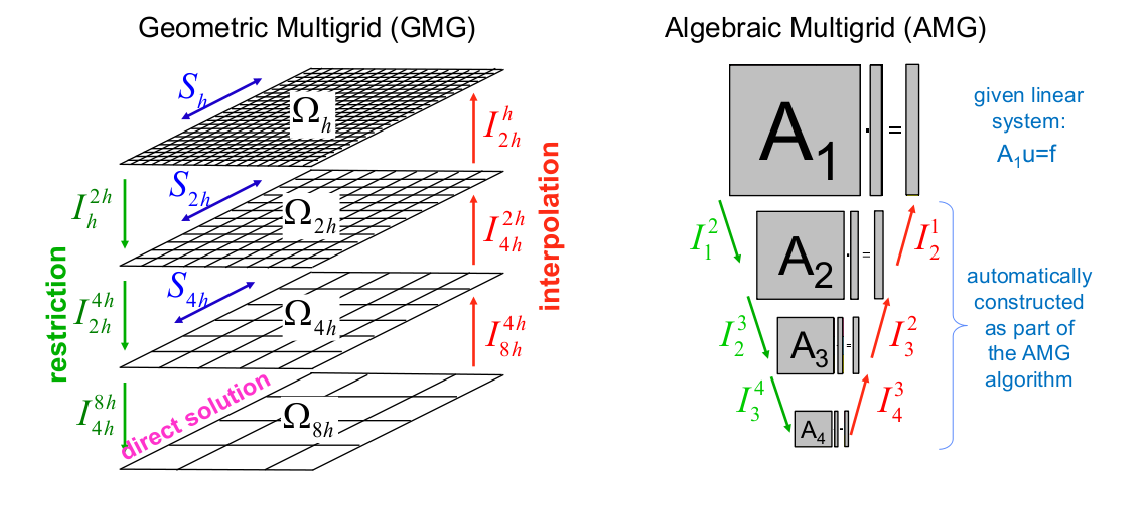
\includegraphics[width=1\textwidth]{resultados/GMGxAMG}
\caption{Comparison of Geometrical and Algebraic Multigrid approaches (from \cite{Trottenberg2001}).}
\label{fig:gmgxamg}
\end{figure}

Mathematically, both approaches can be described in almost the same way, it is just necessary to consider that meshes and nodes are linear system of equation and varibles of this system in AMG, respectively. Therefore, the Multigrid method can be briefly described for both approaches as follows:

Consider the system of equations on the finest level:
\begin{equation} \label{eq:mg1}
A_{f}p_{f} = f_{f}
\end{equation}
where $A_{f}$ is the matrix resultant from the procedure described in section \ref{sc:fem} and the subindex $f$ represent values on the fine level. After performing some iterations with a relaxation method, the error will be smoothed and its residual $r_{h}$ is:
\begin{equation} \label{eq:mg2}
A_{f}\hat{p_{f}} - f_{f} = r_{h}
\end{equation}
where $\hat{p_{f}}$ is the estimated solution for the variable of interest. Subtracting Eq. (\ref{eq:mg2}) from Eq. (\ref{eq:mg1}) yields:
\begin{equation} \label{eq:mg3}
A_{f}p_{f} - A_{f}\hat{p_{f}}= - r_{h}
\end{equation}
and if the operator $A_{h}$ is linear, this equation can be presented as a correction equation:
\begin{equation} \label{eq:mg4}
A_{f}\Delta p_{f}= - r_{h}
\end{equation}

Assuming, as already mentioned, that the high frequency modes of the error were already damped after the relaxation on the fine level, the reminiscent correction error will contain mainly low frequency modes and must be also solved, but in order to achieve this it is necessary to restrict it to a coarser level, where it will present itself as a high frequency mode, i.e.
\begin{equation} \label{eq:mg5}
A_{c}\Delta p_{c}= - I_{f}^{c}r_{f}
\end{equation}
In Eq. (\ref{eq:mg5}) $I_{f}^{c}$ represents the restriction operator, which transfer values from the residual in the fine level $f$ to the coarse level $c$. Once Eq. \ref{eq:mg5} is solved by means of an adequate solver (many times a direct solver will suffice, as this level presents lower storage and computation requirements), its solution can be interpolated back to the fine level using a prolongation operator $I_{c}^{f}$ and the original approximation on the fine level can then be corrected:
\begin{equation} \label{eq:mg6}
\hat{p_{f}^{\phantom{.}\ast}} = \hat{p_{f}} + I_{c}^{f} \Delta p_{c}
\end{equation}
where $\hat{p_{f}^{\phantom{.}\ast}}$ is the updated solution on the fine level. It is important to notice that this procedure is intrinsically recursive, so that the system on the coarse level could be seen as a new fine level, being itself smoothed again until some level is reached where the contributions of the corrections on the coarse levels are taken back to their respective fine levels. There are various schemes to handle this strategy, among them are the V-,W- and F-Cycle. Figure \ref{fig:mgcycles} shows a graphical representation of these cycles on a 4-level multigrid solution, see \cite{Briggs2000} or \cite{Trottenberg2001} for a detailed explanation of each of these cycles.

\begin{figure} 
\centering
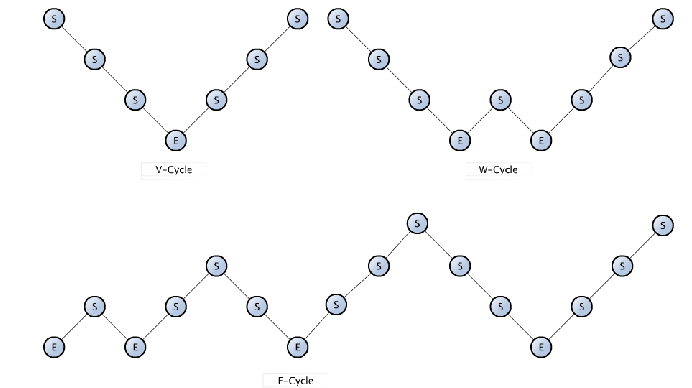
\includegraphics[width=0.9\textwidth]{resultados/MGCycles}
\caption{V- W- and F-Cycles. $S$ represents smoothing and $E$ is the solution on the coarsest level.}
\label{fig:mgcycles}
\end{figure}

\section{AUTOMATED CODING}
All the computational tools described in this work present great challenges not only in terms of theoretical understanding but also in terms of software development, as it is of paramount importance to adequately implement these methods in a way that a positive trade-off between generality and performance is found, as these two goals often lead the coding directives to different directions.

For the generation of the code responsible for assembling the matrices and vectors necessary for the finite element analysis of the problem we used the \emph{FEniCS/DOLFIN} library \citep{Logg2010}, which allows the developer to write the linear and bilinear forms presented in Eq. (\ref{eq:galerkin}) using a script written in \emph{Python} in a very high-level way, that resembles the mathematical notation,  and this script is then automatically converted in optimized \emph{C++} code, which can run quite effectively for general problems.
% Explicar com MUITO mais detalhe o DOLFIN

The obtained system of equations from the discretization with help of the \emph{FEniCS/DOLFIN} library was solved in this work using an Algebraic Multigrid (AMG) approach utilizing the \emph{PyAMG} package \citep{Bell2008}, which allows one to access a number of multigrid algorithms already implemented through a \emph{Python} interface. The most CPU-intensive routines of this package are implemented and compiled in \emph{C++} for performance purposes, but the user does not have to interface with this lower-level code.
% Explicar com MUITO mais detalhe o PyAMG

\section{RESULTS}

\subsection{Heterogeneous and Anisotropic Medium}
\label{sc:heterogeneoaniso}
This example considers an anisotropic and heterogeneous medium. It was proposed originally in \cite{Crumpton1995} as a benchmark test for elliptic problems and was also analyzed in other works \citep{Hyman1997, Carvalho2005, Silva2008}. The domain $\Omega$ is a $[-1,1]$ x $[-1,1]$ square with Dirichlet boundary conditions given by the exact solution. The permeability coefficient $K$ is defined as:
\begin{equation} \label{eq:coeffheteroaniso}
K = \left\{ \begin{array}{cc}
  \phantom{\alpha}\left( \begin{array}{cc}
1 & 0 \\
0 & 1
\end{array} \right) & \textrm{if $x \leq 0$}\\
  \alpha\left( \begin{array}{ll}
2 & 1 \\
1 & 2
\end{array} \right) & \textrm{if $x > 0$}
  \end{array} \right.
\end{equation}
where $\alpha$ is a parameter used to define the discontinuity intensity in $x = 0$.

The analytical solution (and Dirichlet condition for the boundaries) is given by:
\begin{equation} \label{eq:heteroaniso}
p(x,y) = \left\{ \begin{array}{ll}
  [2\sin(y)+\cos(y)]\alpha x + \sin(y) & \textrm{if $x \leq 0$}\\
  \alpha\exp(x)\sin(y) & \textrm{if $x > 0$}
  \end{array} \right.
\end{equation}
 
Finally, the discontinuous source term is defined as:
\begin{equation} \label{eq:bcheteroaniso}
q(x,y) = \left\{ \begin{array}{ll}
  [-2\sin(y)-\cos(y)]\alpha x - \sin(y) & \textrm{if $x \leq 0$}\\
  2\alpha\exp(x)\cos(y) & \textrm{if $x > 0$}
  \end{array} \right.
\end{equation}

For the problem resolution and convergence rates calculation, it was considered a sequence of successive refined meshes with approximate dimensions of $(8x8)$, $(16x16)$, $(32x32)$, $(64x64)$ e $(128x128)$.
The unstructured mesh used for $N \simeq 8$ and the sub-domains boundary in $x=0$ are showed in Fig. \ref{fig:HeterogeneoAnisoMaterials_N=8}.

\begin{figure}
\centering
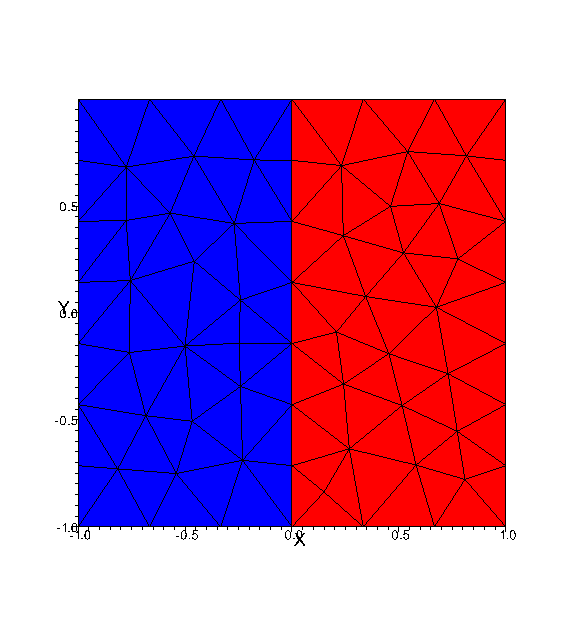
\includegraphics[width=0.45\textwidth]{resultados/HeterogeneoAnisoMaterials_N=8}
\caption{Unstructured mesh with $N \simeq 8$ and discontinuity in $x=0$ for the heterogeneous and anisotropic case.}
\label{fig:HeterogeneoAnisoMaterials_N=8}
\end{figure}

The discontinuity effect on line $x=0$ can be observed in Fig. \ref{fig:HeterogeneoAnisoContour_N=64}, as well as the increase in its intensity as the $\alpha$ parameter is changed. The error maximum and $L2$ norms of the numerical solution when compared to the analytical one are presented on Table \ref{tab:heteroiso}, where can be observed that higher values for the discontinuity in tensor $K$ between the sub-domains implies in an increase of the absolute values obtained for the errors.

\begin{figure}
\centering
\subfigure[$\alpha=1$]{
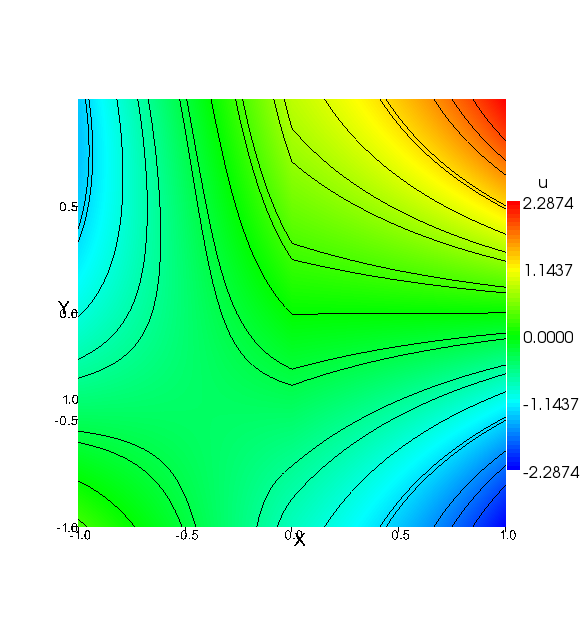
\includegraphics[width=0.45\textwidth]{resultados/HeterogeneoAnisoContour_N=64_alpha=1}
}
\quad
\subfigure[$\alpha=10$]{
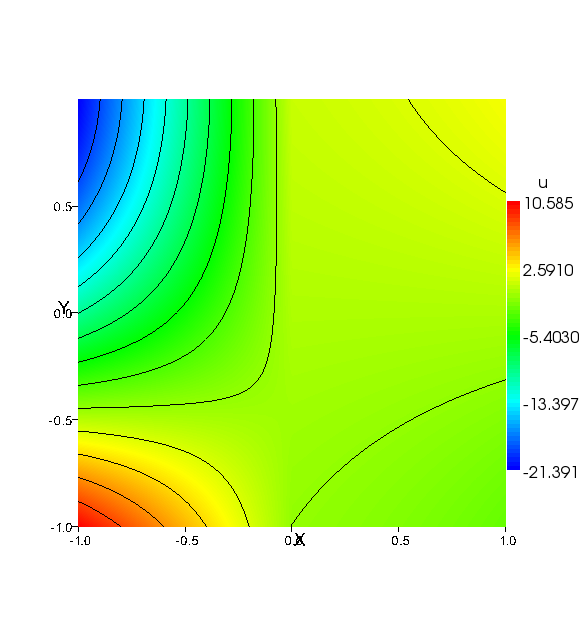
\includegraphics[width=0.45\textwidth]{resultados/HeterogeneoAnisoContour_N=64_alpha=10}
}
\quad
\subfigure[$\alpha=100$]{
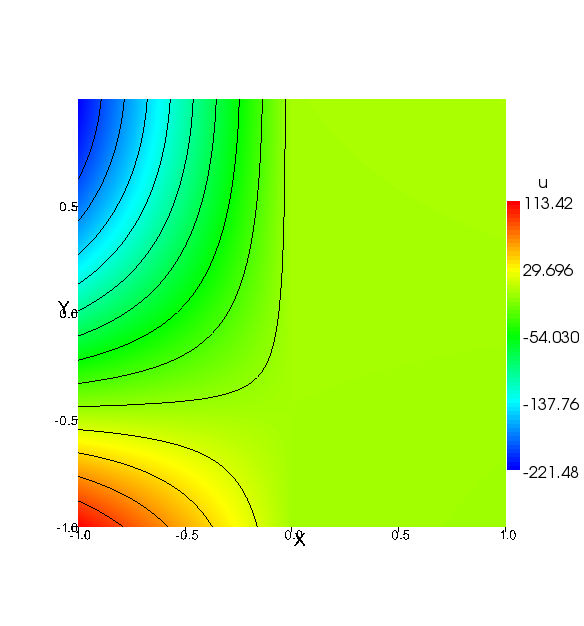
\includegraphics[width=0.45\textwidth]{resultados/HeterogeneoAnisoContour_N=64_alpha=100}
}
\quad
\subfigure[$\alpha=1000$]{
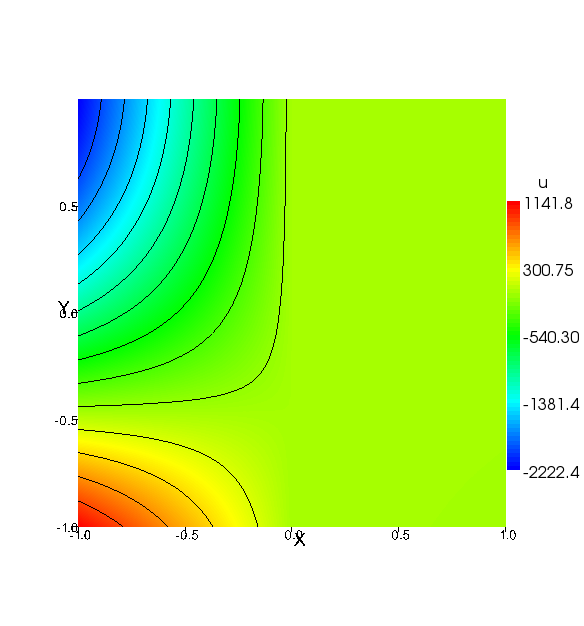
\includegraphics[width=0.45\textwidth]{resultados/HeterogeneoAnisoContour_N=64_alpha=1000}
}
\caption{Scalar pressure field obtained for different discontinuity factors $\alpha$ using the Standard Galerkin FEM in a 64x64 mesh of linear triangles.}
\label{fig:HeterogeneoAnisoContour_N=64}
\end{figure}

\begin{table}
\caption{Error norm and convergence rates for anisotropic and heterogeneous case.}
\centering
\subtable[$\alpha=1$]{
	\begin{tabular}{|c|c|c|c|c|}
	\hline N & \vert\vert E_{max}\vert\vert & q_{max} & \vert\vert E_{L2}\vert\vert & q_{L2} \\
	\hline
	\hline 8 & 5.4e-02 & --- & 4.5e-02 & --- \\ 
	\hline 16 & 2.7e-02 & 0.99 & 2.0e-02 & 1.1 \\ 
	\hline 32 & 1.3e-02 & 1.02 & 9.8e-03 & 1.05 \\ 
	\hline 64 & 6.6e-03 & 1.02 & 4.8e-03 & 1.02 \\ 
	\hline 128 & 3.2e-03 & 1.02 & 2.4e-03 & 1.00 \\ 
	\hline 
	\end{tabular}
	\label{tab:heteroiso1}
}
\qquad\qquad
\subtable[$\alpha=10$]{
	\begin{tabular}{|c|c|c|c|c|}
	\hline N & \vert\vert E_{max}\vert\vert & q_{max} & \vert\vert E_{L2}\vert\vert & q_{L2} \\
	\hline
	\hline 8 & 9.2e-02 & --- & 1.8e-01 & --- \\ 
	\hline 16 & 3.8e-02 & 1.3 & 5.2e-02 & 1.78 \\ 
	\hline 32 & 1.9e-02 & 1.02 & 1.8e-02 & 1.52 \\ 
	\hline 64 & 9.2e-03 & 1.02 & 7.7e-03 & 1.24 \\ 
	\hline 128 & 4.6e-03 & 1.00 & 3.6e-03 & 1.08 \\ 
	\hline 
	\end{tabular}
	\label{tab:heteroiso10}
}
\qquad\qquad
\subtable[$\alpha=100$]{
	\begin{tabular}{|c|c|c|c|c|}
	\hline N & \vert\vert E_{max}\vert\vert & q_{max} & \vert\vert E_{L2}\vert\vert & q_{L2} \\
	\hline
	\hline 8 & 8.6e-01 & --- & 1.7e-00 & --- \\ 
	\hline 16 & 2.9e-01 & 1.59 & 4.3e-01 & 1.98 \\ 
	\hline 32 & 8.8e-02 & 1.70 & 1.1e-01 & 1.98 \\ 
	\hline 64 & 2.5e-02 & 1.79 & 2.8e-02 & 1.94 \\ 
	\hline 128 & 7.2e-03 & 1.81 & 7.9e-03 & 1.84 \\ 
	\hline 
	\end{tabular}
	\label{tab:heteroiso1000}
}
\qquad\qquad
\subtable[$\alpha=1000$]{
	\begin{tabular}{|c|c|c|c|c|}
	\hline N & \vert\vert E_{max}\vert\vert & q_{max} & \vert\vert E_{L2}\vert\vert & q_{L2} \\
	\hline
	\hline 8 & 8.8e-00 & --- & 1.7e+01 & --- \\ 
	\hline 16 & 2.9e-00 & 1.58 & 4.3e-00 & 1.98 \\ 
	\hline 32 & 9.2e-01 & 1.68 & 1.1e-00 & 2.0 \\ 
	\hline 64 & 2.7e-01 & 1.74 & 2.7e-01 & 1.99 \\ 
	\hline 128 & 7.9e-02 & 1.79 & 6.8e-02 & 1.99 \\ 
	\hline 
	\end{tabular}
	\label{tab:heteroiso1000}
}
\label{tab:heteroiso}
\end{table}

An interesting point to be noted is that the values obtained for the numerical solution errors present a convergence rate around 1 for $\alpha = 1$ and $10$, whereas this rate approaches 2 when the discontinuity parameter is increased ($\alpha = 100$ and $1000$).
Comparing this results with those in the references \citep{Crumpton1995,Hyman1997,Carvalho2005,Silva2008}, we notice that methods which perform a local evaluation of the fluxes tend to a convergence rate of 2nd order, while those which work just with the nodal variable (in this case, $p(x,y)$) present a convergence for the error between 1st and 2nd order, in both maximum and $L2$ norms.
One aspect that can contribute for the understanding of this behavior is the error distribution along the domain for various $\alpha$ values. In Fig. \ref{fig:HeterogeneoAnisoError_N=64} can be seen that the error varies smoothly for $\alpha = 1$ and $\alpha = 10$, being concentrated in the discontinuity region, with $x=0$, between the sub-domains. On the other hand, for $\alpha = 100$ e $\alpha = 1000$ the error presents some high frequency modes located mainly in one sub-domain.
This behavior can be explained by the fact that just increasing the $\alpha$ values implies in a higher discontinuity while maintaining the same mesh size, what can be seen as equivalent to keeping the same $\alpha$ and coarsening the mesh, leading to error components with higher frequency modes, independent of its absolute values \citep{Trottenberg2001}.

\begin{figure}
\centering
\subfigure[$\alpha=1$]{
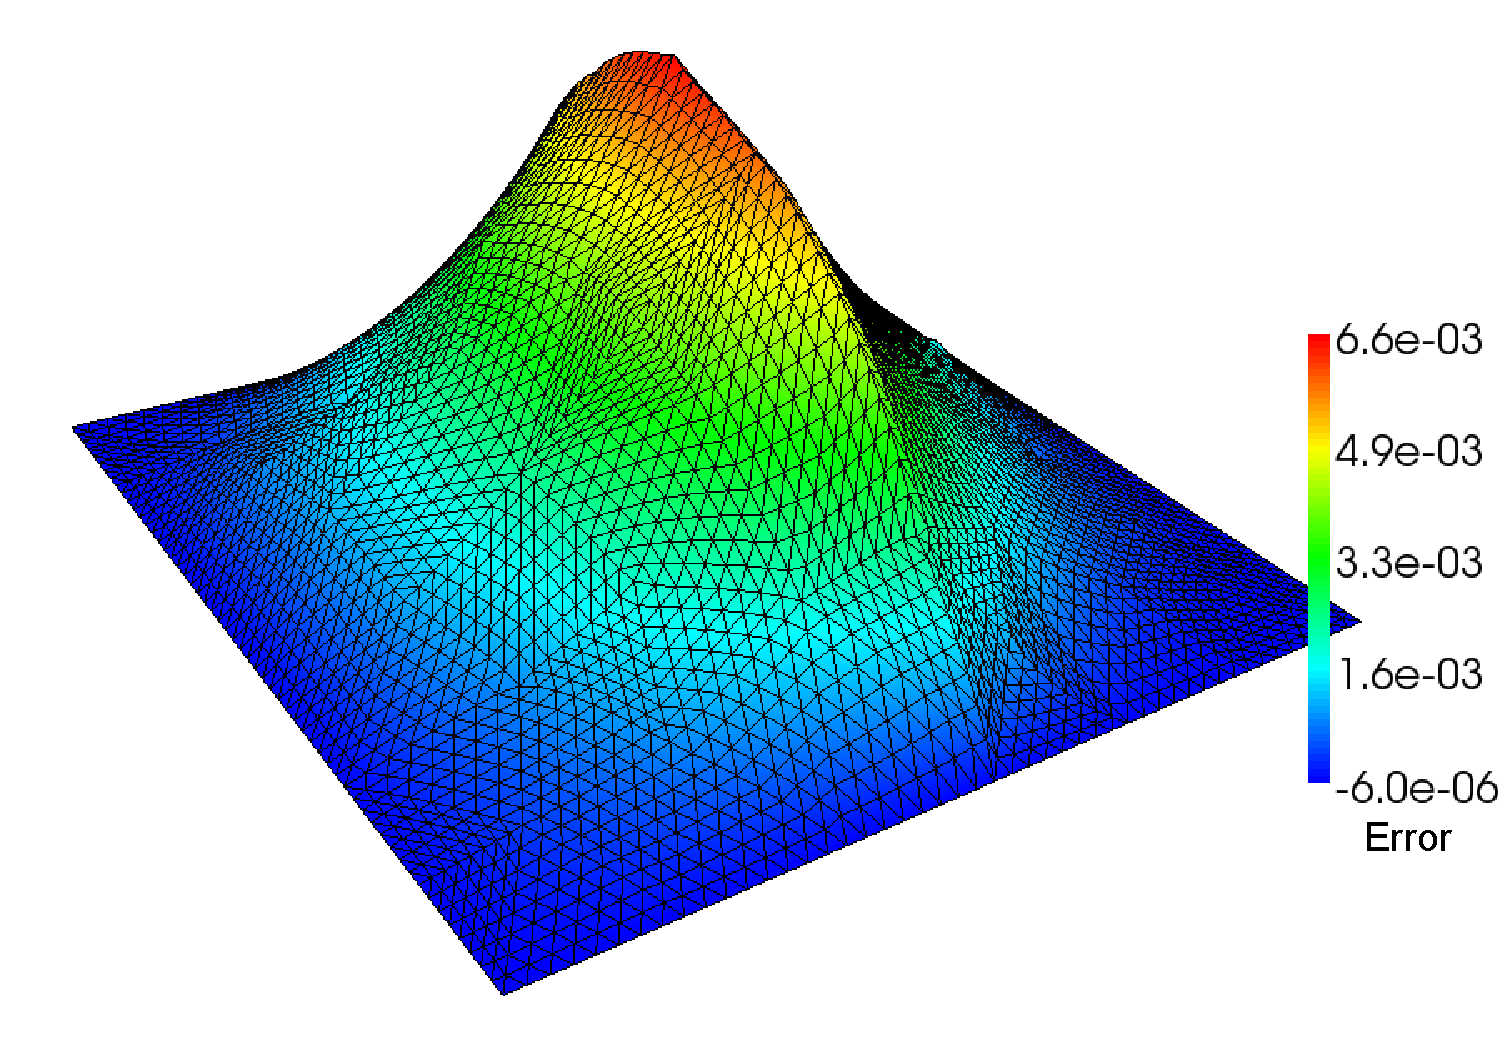
\includegraphics[width=0.45\textwidth]{resultados/HeterogeneoAnisoError_N=64_alpha=1}
}
\quad
\subfigure[$\alpha=10$]{
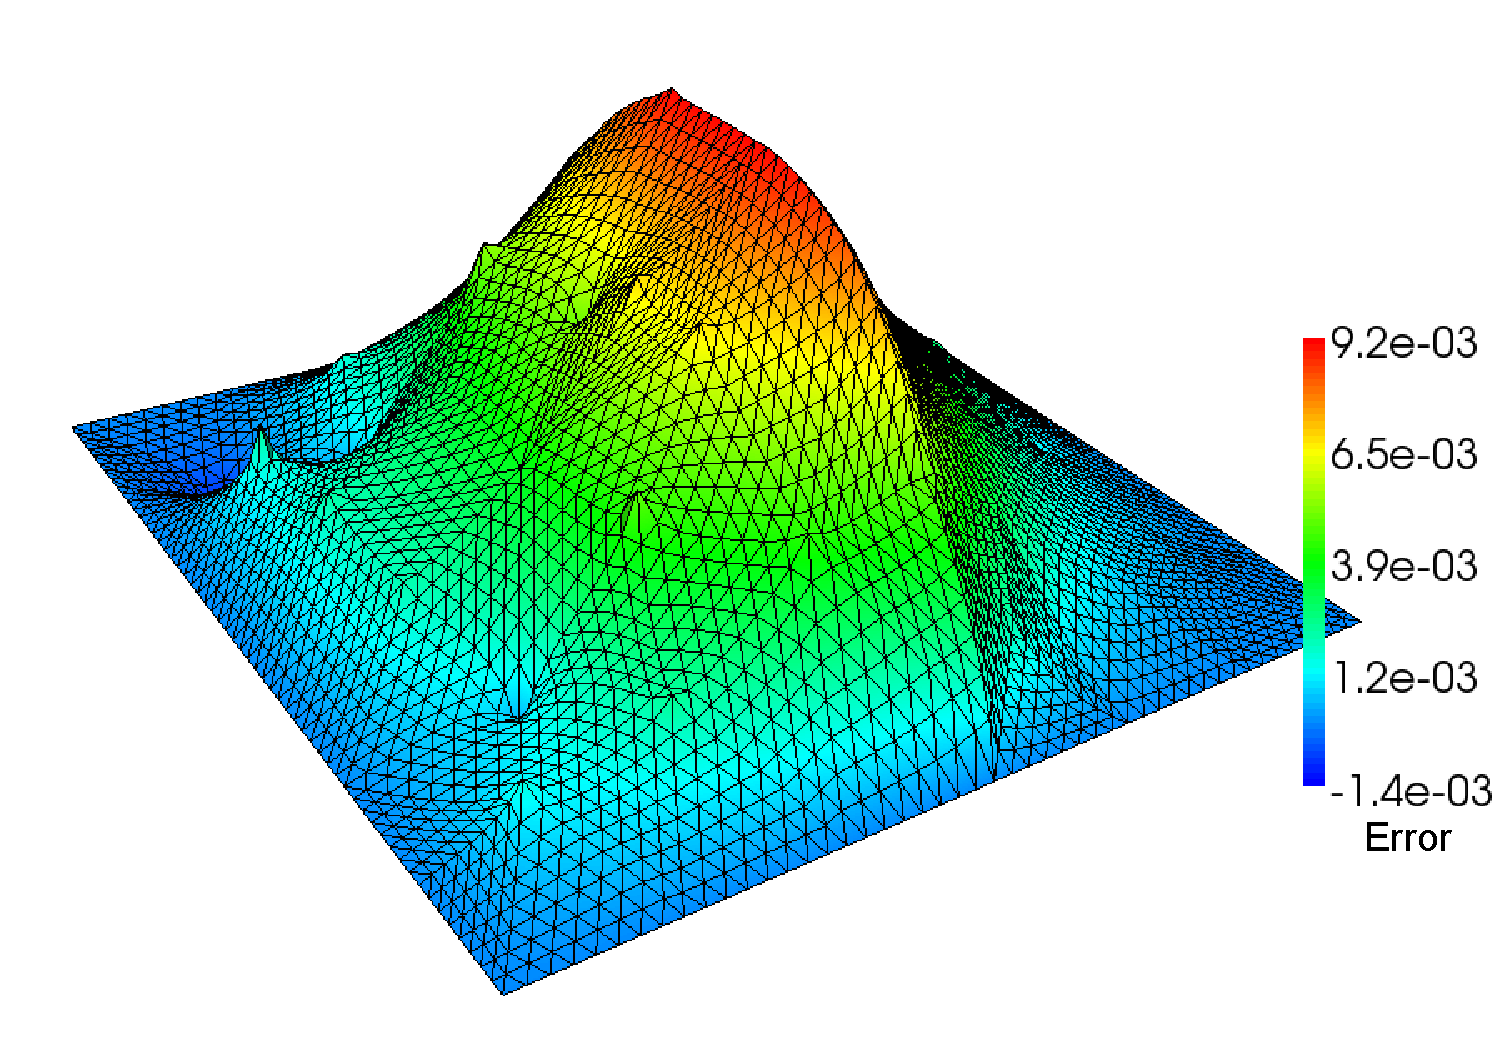
\includegraphics[width=0.45\textwidth]{resultados/HeterogeneoAnisoError_N=64_alpha=10}
}
\quad
\subfigure[$\alpha=100$]{
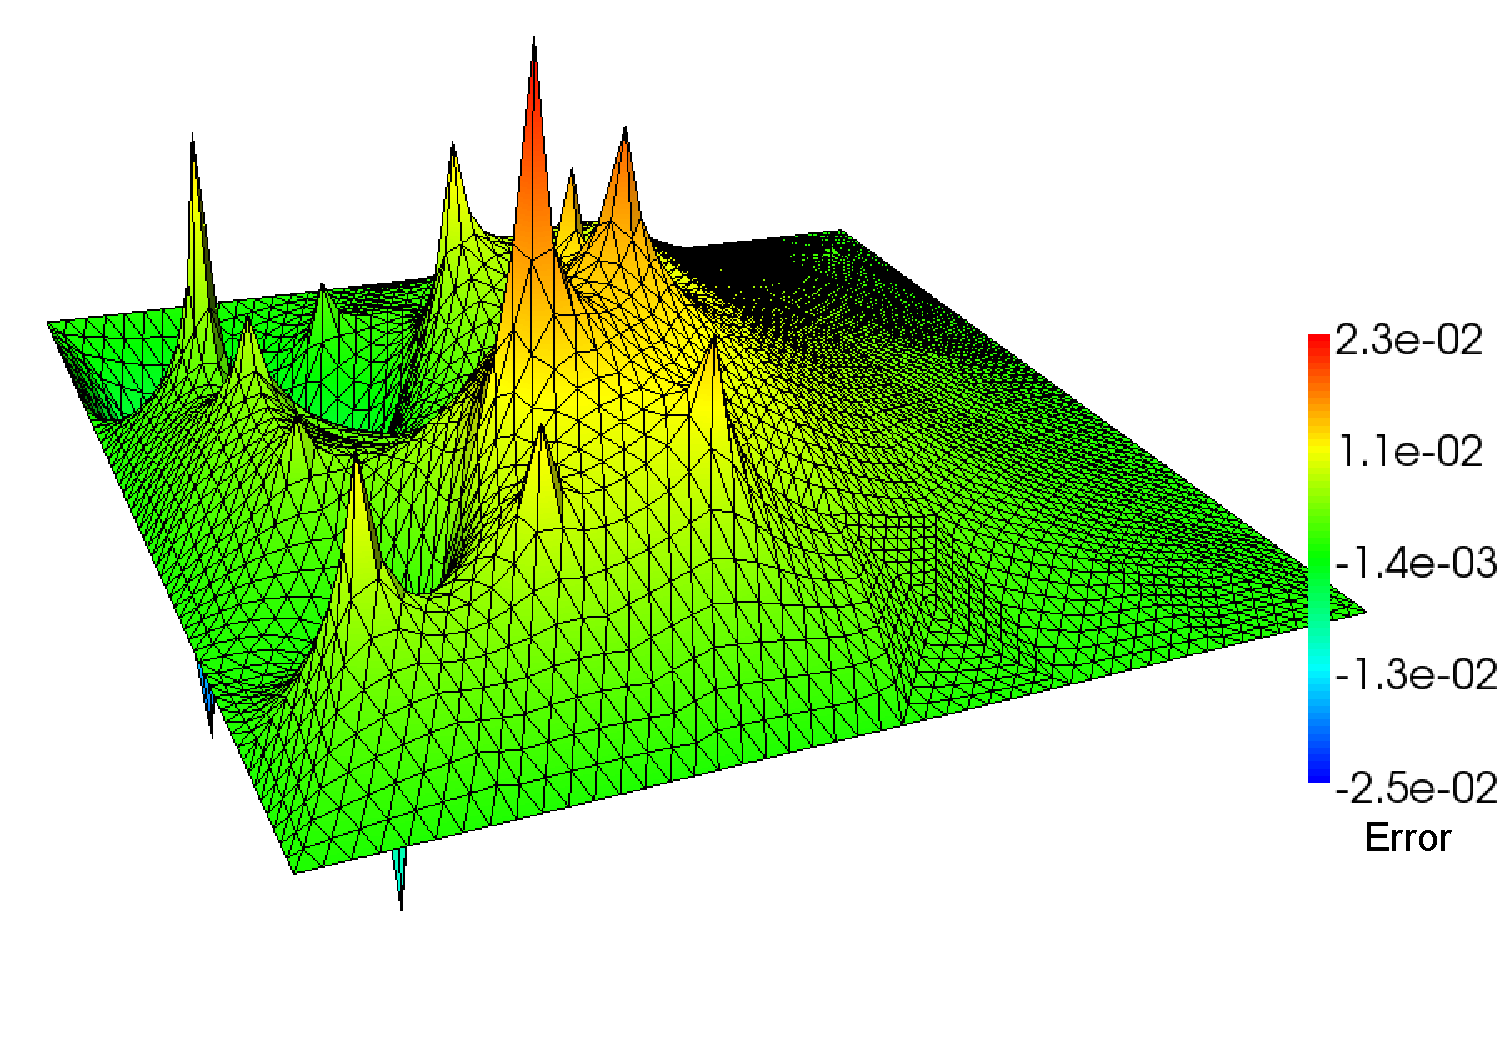
\includegraphics[width=0.45\textwidth]{resultados/HeterogeneoAnisoError_N=64_alpha=100}
}
\quad
\subfigure[$\alpha=1000$]{
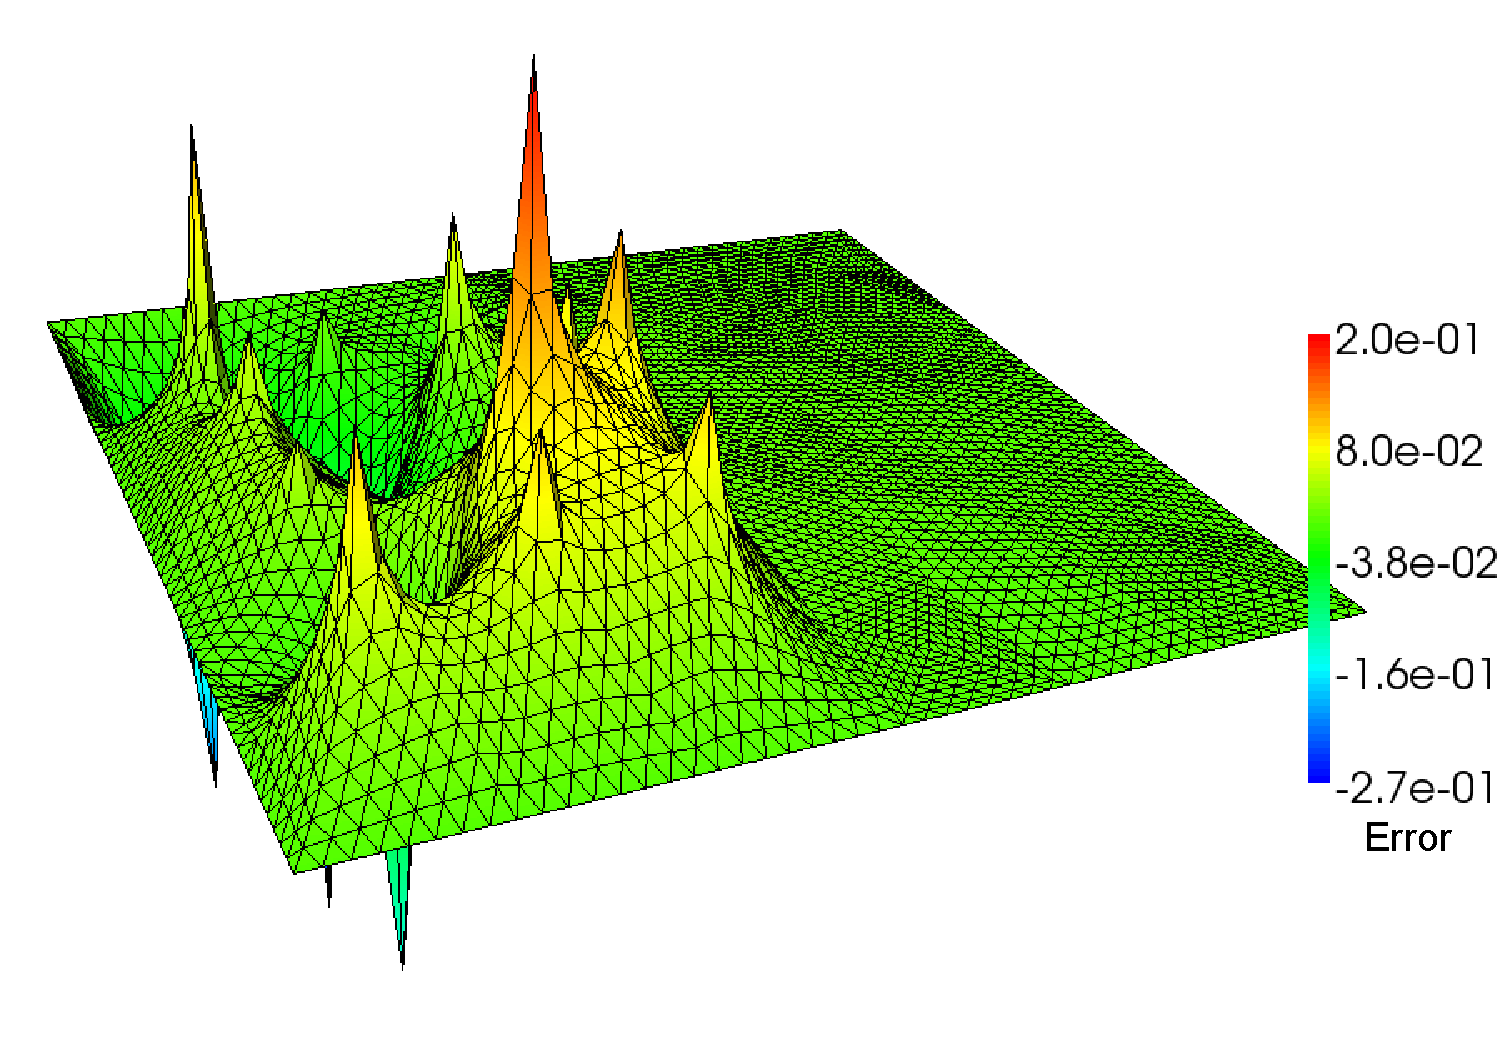
\includegraphics[width=0.45\textwidth]{resultados/HeterogeneoAnisoError_N=64_alpha=1000}
}
\caption{Anisotropic and heterogenous case. Error distribution for $N \simeq 64$ mesh of linear triangles.}
\label{fig:HeterogeneoAnisoError_N=64}
\end{figure}

The performance of various methods for the solution of the linear system of equations were also compared. Naturally, as this problem is represented by a symmetric positive-definite matrix, it would be a candidate to be solved by conjugated gradient-type methods, whether as stand-alone or as preconditioner with an algebraic multigrid methods. Nonetheless, the following combinations for iterative methods were experimented for this problem:
\begin{itemize}
\item Conjugated Gradients (CG) method applied as stand-alone.
\item Generalized Minimal Residual Method (GMRES) applied as stand-alone.
\item Algebraic Multigrid (AMG) applied as stand-alone.
\item Algebraic Multigrid (AMG) as preconditioner for the Conjugated Gradients method (AMG+CG).
\item Algebraic Multigrid (AMG) as preconditioner for the Generalized Minimal Residual Method (AMG+GMRES).
\end{itemize}

For this numerical experiment, it was considered a 64x64 mesh of linear triangles. The stopping criterion for all methods was a tolerance of $\epsilon = 10^{-10}$, with a maximum number of 200 iterations. The $V$ cycle with a 4-meshes hierarchy was considered for the AMG method.
A residual evolution against iteration number graphic is shown in Fig. \ref{fig:residualHeterogeneoAniso_N=64_alpha=1}, where it can be observed the superiority of multigrid-based methods for this kind of elliptic problem, as even in the presence of heterogenity and anisotropy the AMG stand alone stopped by the maximum number of iterations (200).

\begin{figure}
\centering
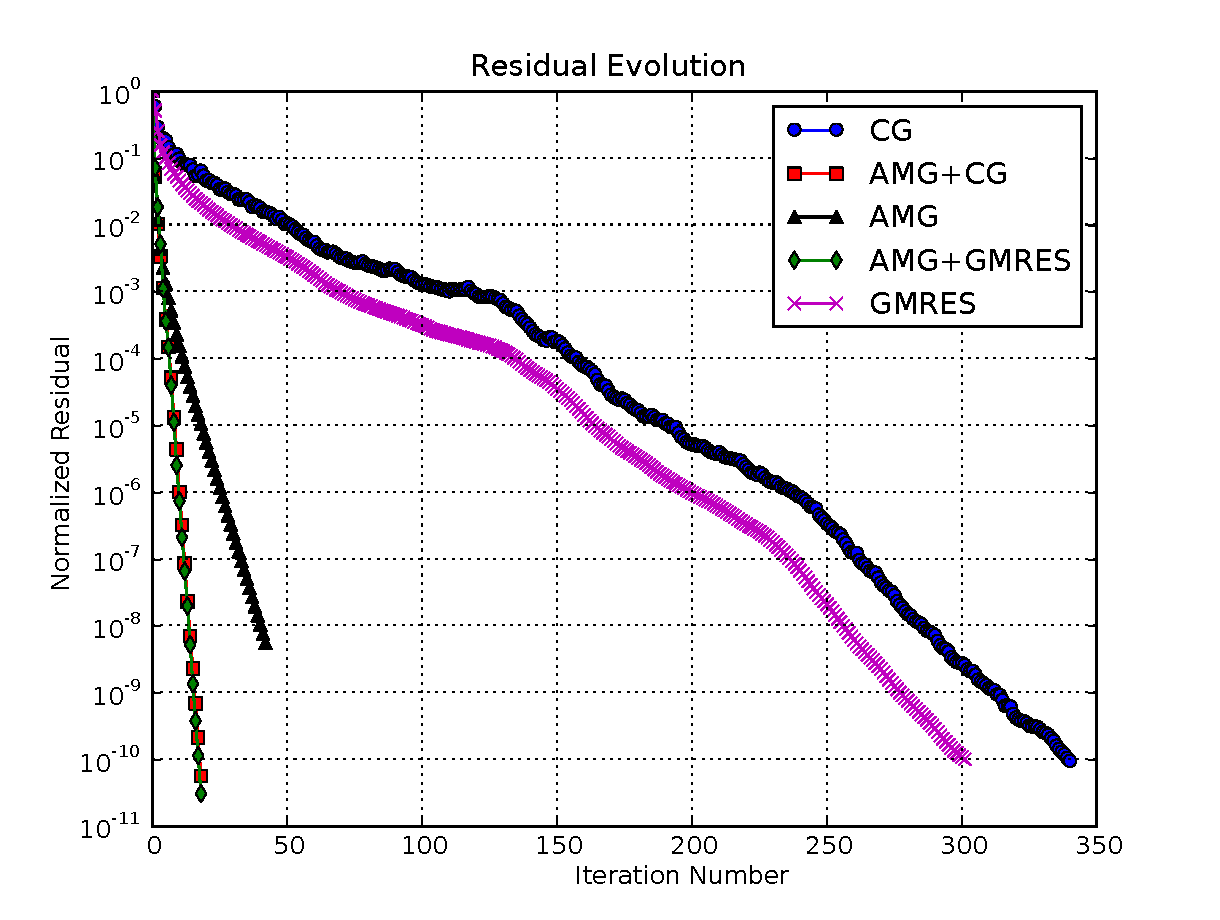
\includegraphics[width=0.7\textwidth]{resultados/residualHeterogeneoAniso_N=64_alpha=1_en}
\caption{Anisotropic and heterogenous case. Residual evolution comparison for $N \simeq 64$ mesh of linear triangles with $\alpha = 1$.}
\label{fig:residualHeterogeneoAniso_N=64_alpha=1}
\end{figure}

\section{CONCLUSIONS}
In this work, a procedure for the solution of the pressure equation in heterogeneous and anisotropic porous media was presented. The PDEs resultant from the mathematical modeling were solved using a Standard Galerkin Finite Element Method approach. In order to accelerate the convergence of the resultant system of equations, an Algebraic Multigrid method was employed, both as stand-alone and as a preconditioner to other solvers. As this kind of numerical framework normally imply in a great time-effort in developing the computational tools that implement them, this work used some available open source libraries in order to automate the generation of low-level code based on some high-level description of the problem. This showed to be a very efficient work methodology, as it allowed to experiment more with the problem in question in less time, because the developer spares time that would be used in "administrative" coding tasks. The results obtained for a model example showed the good performance of the proposed procedure, as the solution converged even for a heterogeneous and highly anisotropic problem. A future work, which is already in progress, will be the solution of the saturation equation associated with the pressure by means of the velocity. The pressure-velocity equation will be solved using a mixed FEM and the saturation equation using a Petrov-Galerkin FEM.


\subsection*{\textit{Acknowledgments}}

\noindent The authors would like to thank the Funda��o de Amparo a Ci�ncia do Estado de Pernambuco (FACEPE) for the financial support during part of the development of this work.

\bibliography{cilamce2011paper}
\end{document}

